\documentclass{article}
\usepackage{etoolbox}
\usepackage{graphicx}
\usepackage{amsmath}

\ifdef{\myoutput}{}{\def\myoutput{concept}}
\ifdef{\myversion}{}{\def\myversion{1}}

\usepackage[output=\myoutput
,numberofversions=4
,version=\myversion
,seed=4
,randomizequestions=true
,randomizeanswers=true
,writeRfile=true
]{mcexam}

\usepackage[margin=0.95in]{geometry}
\usepackage{multicol}

\usepackage{fancyhdr,lastpage}
\pagestyle{fancy}
\fancyhf{}
\renewcommand{\headrulewidth}{1pt} 
\renewcommand{\footrulewidth}{1pt}
\lfoot{\mctheversion}
\rfoot{Page \thepage\ of \pageref{LastPage}}
\lhead{Quiz 10.2 \mctheversion \\ MAT 2000: Introduction to Statistics}
\rhead{Name Print): \hspace{2.5 in}}

\usepackage{calc}
\renewenvironment{setmcquestion}
{\begin{minipage}[t]{\linewidth-\labelwidth}}
	{\end{minipage}\par}
	
\renewenvironment{setmcquestioninstruction}
{\begin{minipage}{\textwidth}}
	{\end{minipage}}
	
\renewenvironment{setmcanswers}{}{}
\setlist[setmcquestions]{label=\mcquestionlabelfmt{*}.
	,ref=\mcquestionlabelfmt{*}
	,itemsep=0.5\baselineskip
	,topsep=1\baselineskip
}

\renewcommand\mcversionlabelfmt[1]{\arabic{#1}}

%copy-pasting from MS Word, use regex to find [\*]*[a-d]\. and replace with \answer 

\raggedbottom

\begin{document}
	Circle the correct answer for each question.  If you're unsure, you can write numbers 1, 2, 3, etc. next to the choices to get partial credit.  Questions refer to the nonindented paragraph above unless otherwise stated.\\[.5cm]
	
	\begin{mcquestions}
		
		\question The two graphs, A and B, show dotplots from two different data sets. Suppose I want to compare the means in A and do another comparison of means in B. For each case an F-statistic is computed. Which of the following will be true about these statistics?
		\begin{center}
			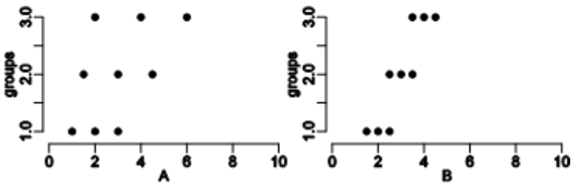
\includegraphics[width = 0.75\textwidth]{images/q-10-2-1.png}
		\end{center}
		\begin{mcanswerslist}
			\answer The F-statistic is the same in A and B.
			\answer The F-statistic is larger in A than in B.
			\answer[correct] The F-statistic is smaller in A than in B.
			\answer We cannot tell if the F-statistic will be larger in A or B.
		\end{mcanswerslist}
		
		\question An experiment is conducted which randomly places students into one of three treatment groups: (1) those students who will take a test that is printed on white paper, (2) those students who will take the same test, but printed on red paper, and (3) those who will take the same test, but printed on blue paper. The researcher analyzes the data using ANOVA in order to compare the average scores in the three groups looking for evidence that the average score is different on at least one of the three tests. Assume that at least one group really is different when answering the following question.
		
		As the size of the sample in each group increases, all else remaining the same, what will be the impact on the strength of evidence for finding a difference in the average scores on the three exams?
		
		\begin{mcanswerslist}
			\answer[correct] There will be more evidence of a difference.
			\answer There will be less evidence of a difference.
			\answer There will be no impact on the strength of evidence of a difference.
			\answer There is not enough information to tell.
		\end{mcanswerslist}
		
		\begin{mcquestioninstruction}
			A British study examined whether the type of background music playing in a restaurant affected the amount of money that diners spent on their meals.  The researchers asked a restaurant to alternate silence, popular music, and classical music on successive nights over eighteen days.  Each type of music was played for 6 nights (the order was randomly determined to guard against confounding). The type of music played and the amount spent on food and drinks (in British pounds) for each of 393 customers was recorded. The data are summarized below.
			\begin{center}
				\begin{multicols}{2}
					\begin{tabular}{l|c|c|c|}
						&Sample size&Mean&StDev\\
						Classical&120&24.1&2.30\\
						Pop&142&21.9&2.73\\
						None&131&21.7&3.38\\
						Pooled&393&22.5&2.85
					\end{tabular}
					
					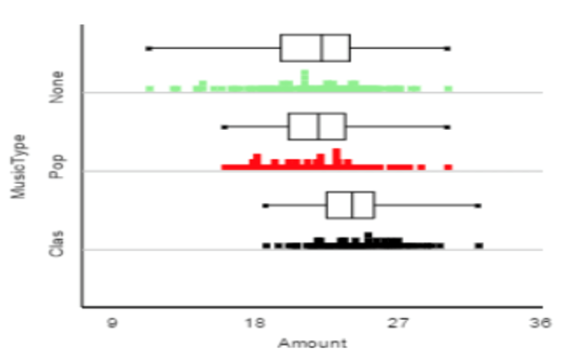
\includegraphics[width=0.5\textwidth]{images/q-10-2-2.png}
				\end{multicols}
			\end{center}
		\end{mcquestioninstruction}
		\question All of the following statements are true for this situation, but one is not a legitimate validity condition.  Which one is not the real validity condition?
		\begin{mcanswerslist}
			\answer The standard deviations of the sample are approximately equal.
			\answer The sample sizes are all at least 20.
			\answer The sample distributions show no strong skewness.
			\answer[correct] The sample means are all at least 20.
		\end{mcanswerslist}
		
		\question[follow] The p-value for the ANOVA F-test is less than 0.001. How would you interpret this value?
		\begin{mcanswerslist}
			\answer[correct] In less than 0.1\% of all samples, the F-statistic would be as large or larger than the one observed, assuming there is no association between music type and amount spent on food and drinks.
			\answer In less than 0.1\% of all samples, the F-statistic would be as small or smaller than the one observed, assuming there is no association between music type and amount spent on food and drinks.
			\answer In less than 0.1\% of all samples, the F-statistic would be as large or larger than the one observed, assuming there is an association between music type and amount spent on food and drinks.
			\answer In less than 0.1\% of all samples, the F-statistic would be as small or smaller than the one observed, assuming there is an association between music type and amount spent on food and drinks.
		\end{mcanswerslist}
		
		\question When performing an ANOVA F-test, which definition of a p-value is the most accurate?
		\begin{mcanswerslist}
			\answer The p-value is the probability that the observed F-statistic will occur again.
			\answer[correct] If the null hypothesis is true, the p-value is the probability of observing an F-statistic as large or larger than the one actually observed.
			\answer The p-value is the value that an F-statistic must reach in order to be significant under the null hypothesis.
			\answer The p-value is the probability that the null hypothesis is true.
		\end{mcanswerslist}
	\end{mcquestions}
\end{document}